\chapter{Experiments and Results}
\label{chap:experiments}

Experiments for our VMMR system are conducted on a platform with Dual-Core Intel Core i5 (2.9 GHz), 16 GB 1867 MHz DDR3 and MATLAB R2019b.

\section{Pre-processing}
\label{sec:pre-processing}
In the pre-processing stage, Regions Of Interest (ROI) are cropped out, converted to grayscale and scaled to a unified resolution of 140-by-140.

\subsection{Duplicates Removal}
The original dataset contains $2117$ frontal car images in total. 
However, for each distinct car in the dataset, there exist multiple variations, which typically include a coloured non-cropping version, a grayscale downsampled version, as well as a grayscale downsampled and ROI-cropped version.
Duplicates removal are achieved by preversing the coloured non-cropping version of size 640-by-480 only among those variations.
A total of $500$ "original images" are retrieved.

For "peugeot306" and "citroen\_saxo" classes, however, the coloured non-cropping versions are missing.
In that case, the grayscale downsampled and ROI-cropped versions are chosen and both the cropping and converting steps are skipped.


\subsection{Cropping}
In the cropping stage, ROI are cropped out from the "original images".
Locations of number plates in the "original images" have already been pre-labeled.
In this paper, ROI is defined in terms of the width $w$ and the center $(x_c, y_c)$ of the number plate in the image.
Concretely, the rectangle bounding box of ROI is written as $[(x_c-1.4w, y_c-0.7w), ((x_c+1.4w, y_c+0.4w))]$.
An example of ROI cropping is shown in Figure \ref{fig:roi}.

\begin{figure}
\centering
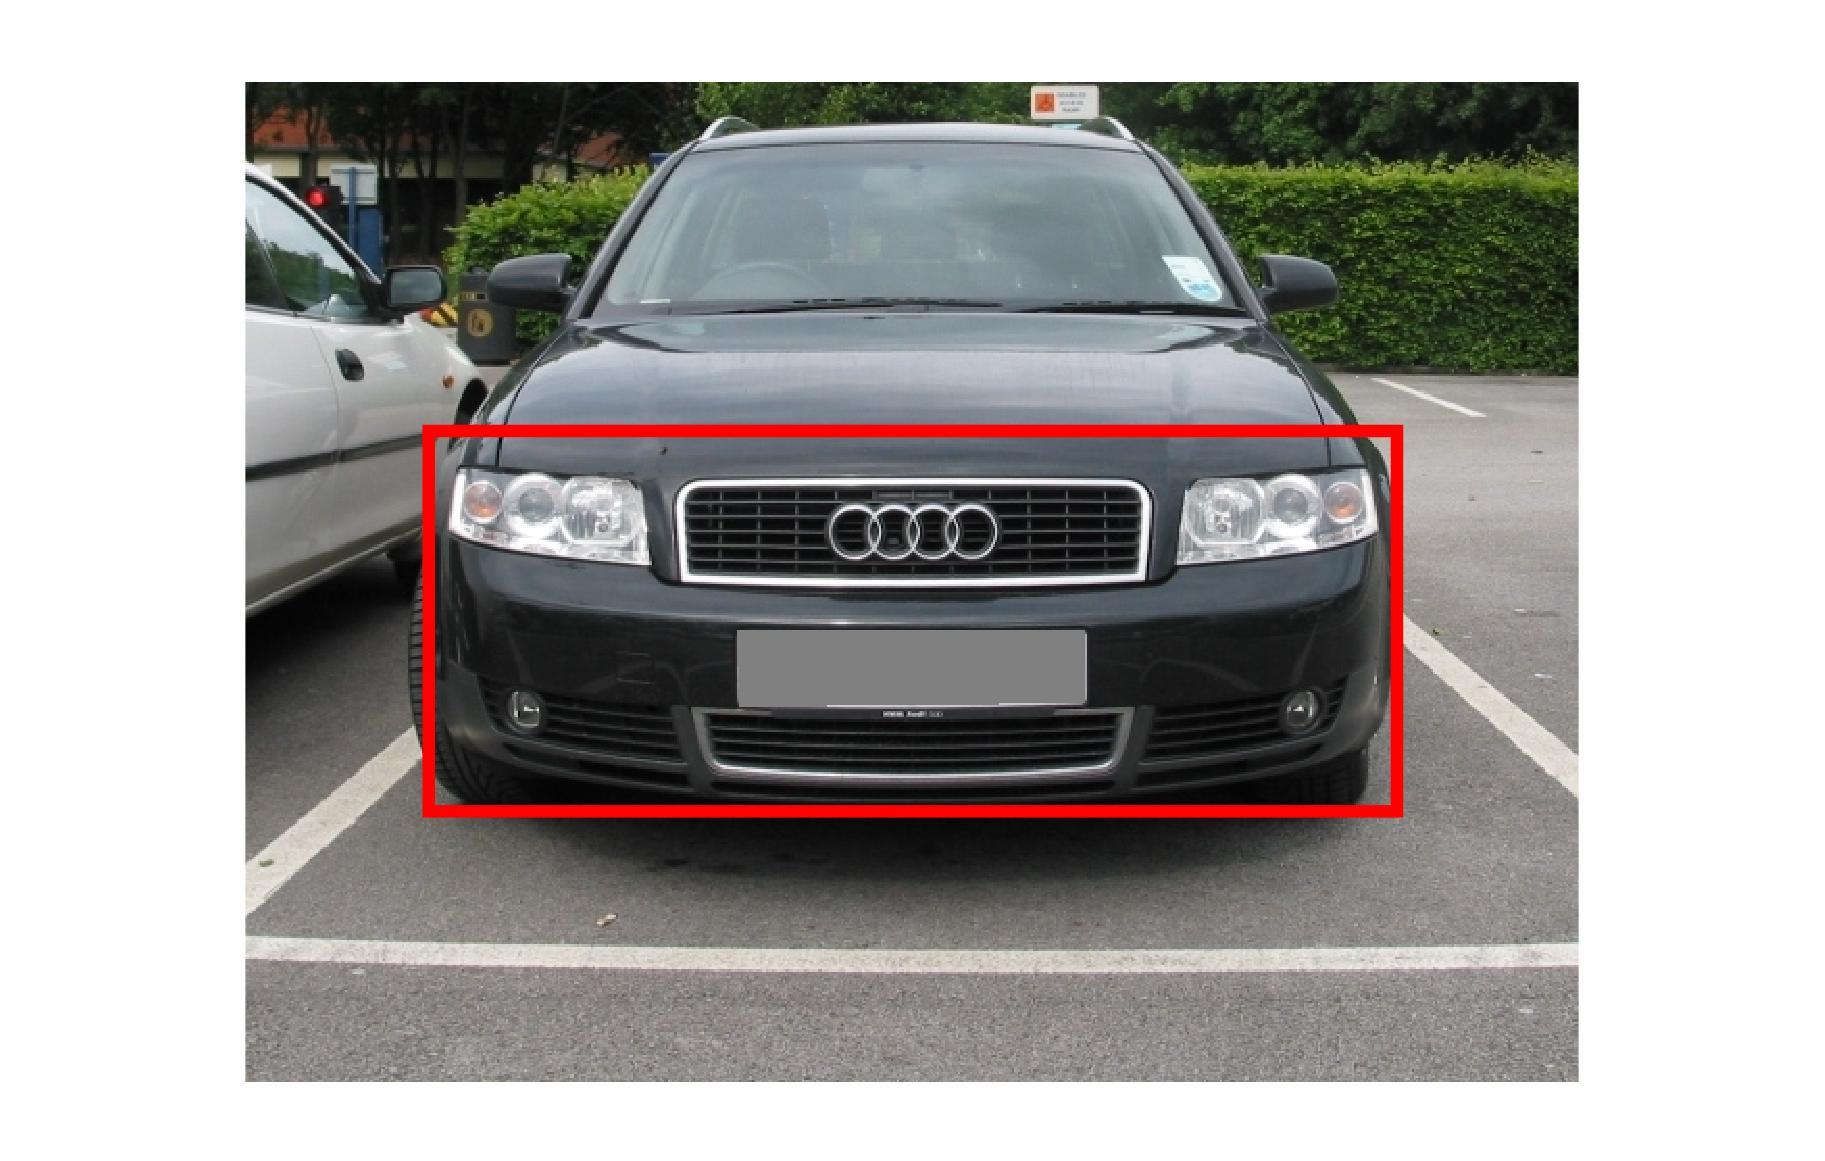
\includegraphics{roi}
\caption{An Example of ROI Cropping on a "Original Image" from "audi\_a4" Class.}
\label{fig:roi}
\end{figure}


\subsection{Converting to Grayscale}
The cropped RGB images are convertted to grayscale image using Formula \ref{eq:rgb2gray}.

\begin{equation}
\label{eq:rgb2gray}
I = 0.2989 R + 0.5870 G + 0.1140 B
\end{equation}

The pre-processed dataset before scaling can be retrieved from GitHub \footnote{https://github.com/daidahao/COP507-Vehicle-Make-Model-Recognition/tree/master/dataset}.

\subsection{Scaling}
All images are scaled to a unified resolution of 140-by-140 at runtime.
A set of scaled image samples for all classes are presented in Figure \ref{fig:classes}.

\section{Cross-Validation}
In our experiments, $5$-fold cross-validation is applied to each model-paramter set.
Accuracy, precision, recall and f1 scores averaged across class are reported for each set.

% \section{Merits of Performance}

\section{Effects of Features Extraction Methods}
\label{sec:effects-fe}
To evaluate the effects of features extraction methods, performance of VMMR systems using Raw Image, SER, SMG, LNHS, BSURF as features are evaluated and compared in Table \ref{tab:features}.
In addition, LNHS and BSURF are evaluated under a variety of parameter set.
The default classification method is SVM and dimensionality reduction is skipped.

\begin{longtable}[]{@{}lllll@{}}
\toprule
& Accuracy (\%) & Precision (\%) & Recall (\%) & F1 Score
(\%)\tabularnewline
\midrule
\endhead
Raw Image & 90.00 & 89.61 & 89.87 & 89.74\tabularnewline
SER & 32.08 & 48.63 & 28.04 & 35.57\tabularnewline
SMG & \textbf{99.62} & \textbf{99.70} & \textbf{99.63} &
\textbf{99.66}\tabularnewline
LNHS (\(d = 1\)) & 3.77 & 3.47 & 4.80 & 4.03\tabularnewline
LNHS (\(d = 2\)) & 36.23 & 35.46 & 34.53 & 34.99\tabularnewline
LNHS (\(d = 3\)) & 88.68 & 89.45 & 89.14 & 89.29\tabularnewline
LNHS (\(d = 4\)) & 99.06 & 99.08 & 98.99 & 99.03\tabularnewline
LNHS (\(d = 5\)) & \textbf{99.62} & 99.62 & 99.58 & 99.60\tabularnewline
LNHS (\(d = 6\)) & 99.43 & 99.37 & 99.42 & 99.39\tabularnewline
LNHS (\(d = 7\)) & 96.23 & 97.44 & 96.62 & 97.03\tabularnewline
BSURF (\(T = 500\)) & 84.34 & 85.38 & 84.01 & 84.69\tabularnewline
BSURF (\(T = 1000\)) & 86.98 & 88.38 & 87.04 & 87.70\tabularnewline
BSURF (\(T = 2000\)) & 90.00 & 91.26 & 90.25 & 90.75\tabularnewline
BSURF (\(T = 4000\)) & 92.45 & 93.83 & 92.85 & 93.34\tabularnewline
BSURF (\(T = 8000\)) & 93.02 & 94.64 & 93.15 & 93.89\tabularnewline
BSURF (\(T = 16000\)) & 93.96 & 95.77 & 94.69 & 95.23\tabularnewline
BSURF (\(T = 32000\)) & 93.96 & 95.62 & 93.55 & 94.57\tabularnewline
\bottomrule
\caption{Performance of VMMR System Using Different Features Extraction Methods.}
\label{tab:features}
\end{longtable}

SER achieves the poorest performance among three simplest features with accuracy score of $32.08\%$. The reason is that edge response are sensitive to noise and directional changes of edges.
On the other hand, SMG performs the best among all features with accuracy score of $99.62\%$.
The reason behind that is that SMG describes the parallel and diagonal components of change in SER and is robust to noise and directional changes of edges.

LNHS with depth of $d = 5$ and length of $1364$ achieves comparable performance to SMG with length of $39200$, having the same accuracy and a lower precision and recall scores.
Deeper LNHS features, however, decrease the performance in all merits.
One explanation for that would be shallower LNHS normalizes Harris corner strengths in a more robust manner.
The deepest quardant of LNHS with $d = 5$ is normalized by the sum of Harris strengths on $76.56$ pixels on average, compared to $4.79$ pixels when $d = 7$.
% Justification

BSURF features achieve poorer performance even when the length of feature vector is $32000$ and close to SMG.

SMG, which outperforms all the other features in all merits, is the default features extraction method in the following sections.

\section{Effects of Classification Methods}
\label{sec:effects-cls}
Performance of VMMR systems using KNN and SVM as classifier are evaluated and compared in Table \ref{tab:classifiers}.
In addition, KNN are evaluated under a different values of $K$.
The default classification method is SMG and dimensionality reduction is skipped.

\begin{longtable}[]{@{}lllll@{}}
\toprule
& Accuracy (\%) & Precision (\%) & Recall (\%) & F1 Score
(\%)\tabularnewline
\midrule
\endhead
KNN (\(K=1\)) & 99.43 & 99.69 & 99.59 & 99.64\tabularnewline
KNN (\(K=3\)) & 99.43 & 99.67 & 99.38 & 99.52\tabularnewline
KNN (\(K=5\)) & \textbf{99.62} & 99.76 & 99.52 & 99.64\tabularnewline
KNN (\(K=7\)) & 99.43 & 99.56 & 99.29 & 99.42\tabularnewline
KNN (\(K=9\)) & 98.87 & 99.20 & 98.78 & 98.99\tabularnewline
SVM & \textbf{99.62} & \textbf{99.77} & \textbf{99.63} &
\textbf{99.70}\tabularnewline
\bottomrule
\caption{Performance of VMMR System Using Different Classification Methods.}
\label{tab:classifiers}
\end{longtable}


KNN model performs best with accuracy of $99.62\%$ when $K = 5$.
There are $2$ main reasons for that. 
First, a larger $K$ value means more neighbours need to be found to support a prediction and thus the classifier is more robust.
Second, some vehicle classes have fewer than $10$ images durning training. Given a image from one of those classes, neighbours of the same class could be inadequate to form a majority.
% Justification

SVM achieves the best performance in all merits with accuracy of $99.62\%$ and F1-Score of $99.70\%$. 
Therefore, SVM is the default classification method for the following sections.

\section{Effects of Dimensionality Reduction Methods}
\label{sec:effects-dim}
Performance of VMMR systems whether using dimensionality reduction are evaluated and compared in Table \ref{tab:pca}.
In addition, PCA is evaluated under different $\sigma$ values.

\begin{longtable}[]{@{}llllll@{}}
\toprule
& Length & Accuracy (\%) & Precision (\%) & Recall (\%) & F1 Score
(\%)\tabularnewline
\midrule
\endhead
Skipped & 39200 & \textbf{99.62} & \textbf{99.77} & 99.63 &
\textbf{99.70}\tabularnewline
PCA (\(\sigma=60\)) & 203 & \textbf{99.62} & 99.66 & \textbf{99.70} &
99.68\tabularnewline
PCA (\(\sigma=70\)) & 270 & \textbf{99.62} & \textbf{99.77} & 99.63 &
\textbf{99.70}\tabularnewline
PCA (\(\sigma=80\)) & 344 & \textbf{99.62} & \textbf{99.77} & 99.63 &
\textbf{99.70}\tabularnewline
PCA (\(\sigma=90\)) & 429 & \textbf{99.62} & \textbf{99.77} & 99.63 &
\textbf{99.70}\tabularnewline
PCA (\(\sigma=95\)) & 476 & \textbf{99.62} & \textbf{99.77} & 99.63 &
\textbf{99.70}\tabularnewline
PCA (\(\sigma=99\)) & 581 & \textbf{99.62} & \textbf{99.77} & 99.63 &
\textbf{99.70}\tabularnewline
\bottomrule
\caption{Performance of VMMR System Using Optional Dimensionality Reduction Method.}
\label{tab:pca}
\end{longtable}

The introduction of dimensionality reduction into our system does not have any effect on the performance when $\sigma$ for PCA is above $70$.
Using a feature vector of length $270$ after PCA produces the same performance of using a full SMG feature vector of length $39200$.
The reason is that SMG on each pixel is highly correlated to neighbours and thus can be dramaitically reduced in dimensionality.


\section{Best Performance}
% on a new dataset

The best performance of our proposed VMMR system is achieved on the dataset when SMG is used for feature extraction, PCA ($\sigma = 70$) for dimensionality reduction and SVM for classification.
The model produces an accuracy score of $99.62\%$, precision of $99.77\%$, recall of $99.62\%$ and F1-score of $99.70\%$.
A confusion matrix of the model is drawn in Figure \ref{fig:confusion}, where predictions are made in $5$-fold cross validation scheme.

\begin{figure}
\centering
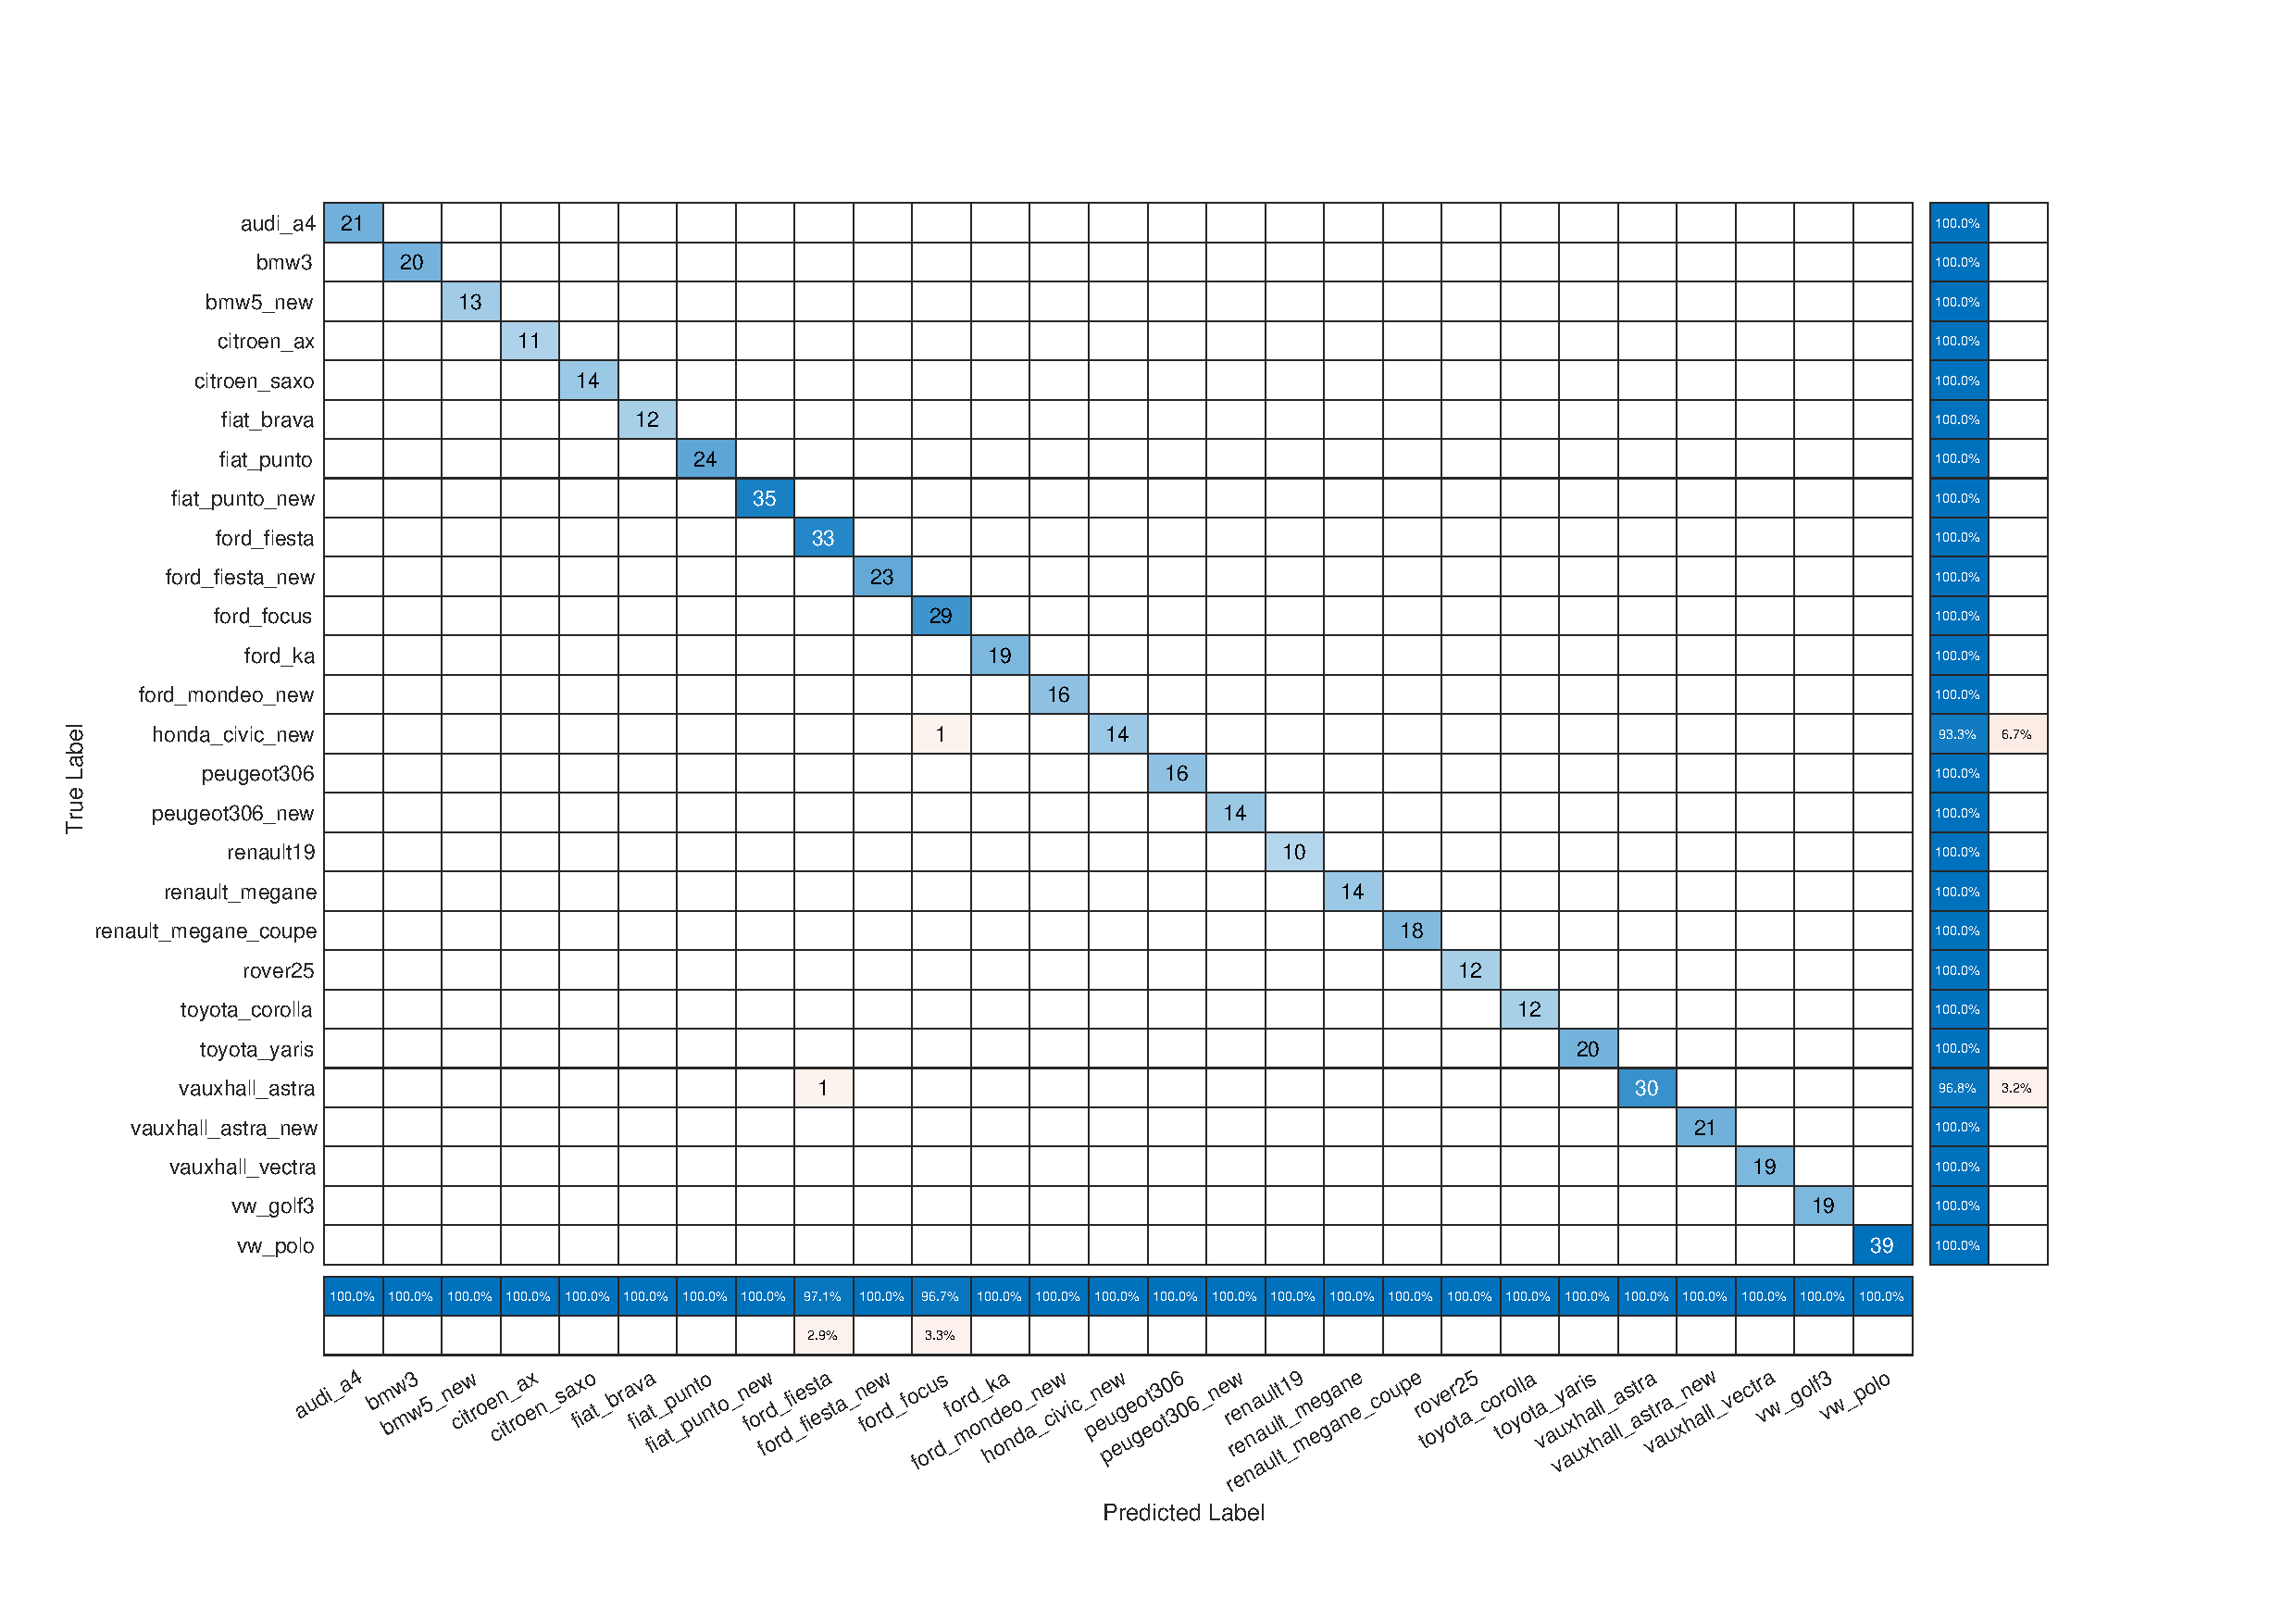
\includegraphics{confusion}
\caption{Confusion Matrix on Corss-Validated Dataset of Our Poposed VMMR System (SMG + PCA + SVM).}
\label{fig:confusion}
\end{figure}

Only $2$ misclassifications are made on the dataset, as presented in Figure \ref{fig:mis}. 

\begin{figure}
\centering
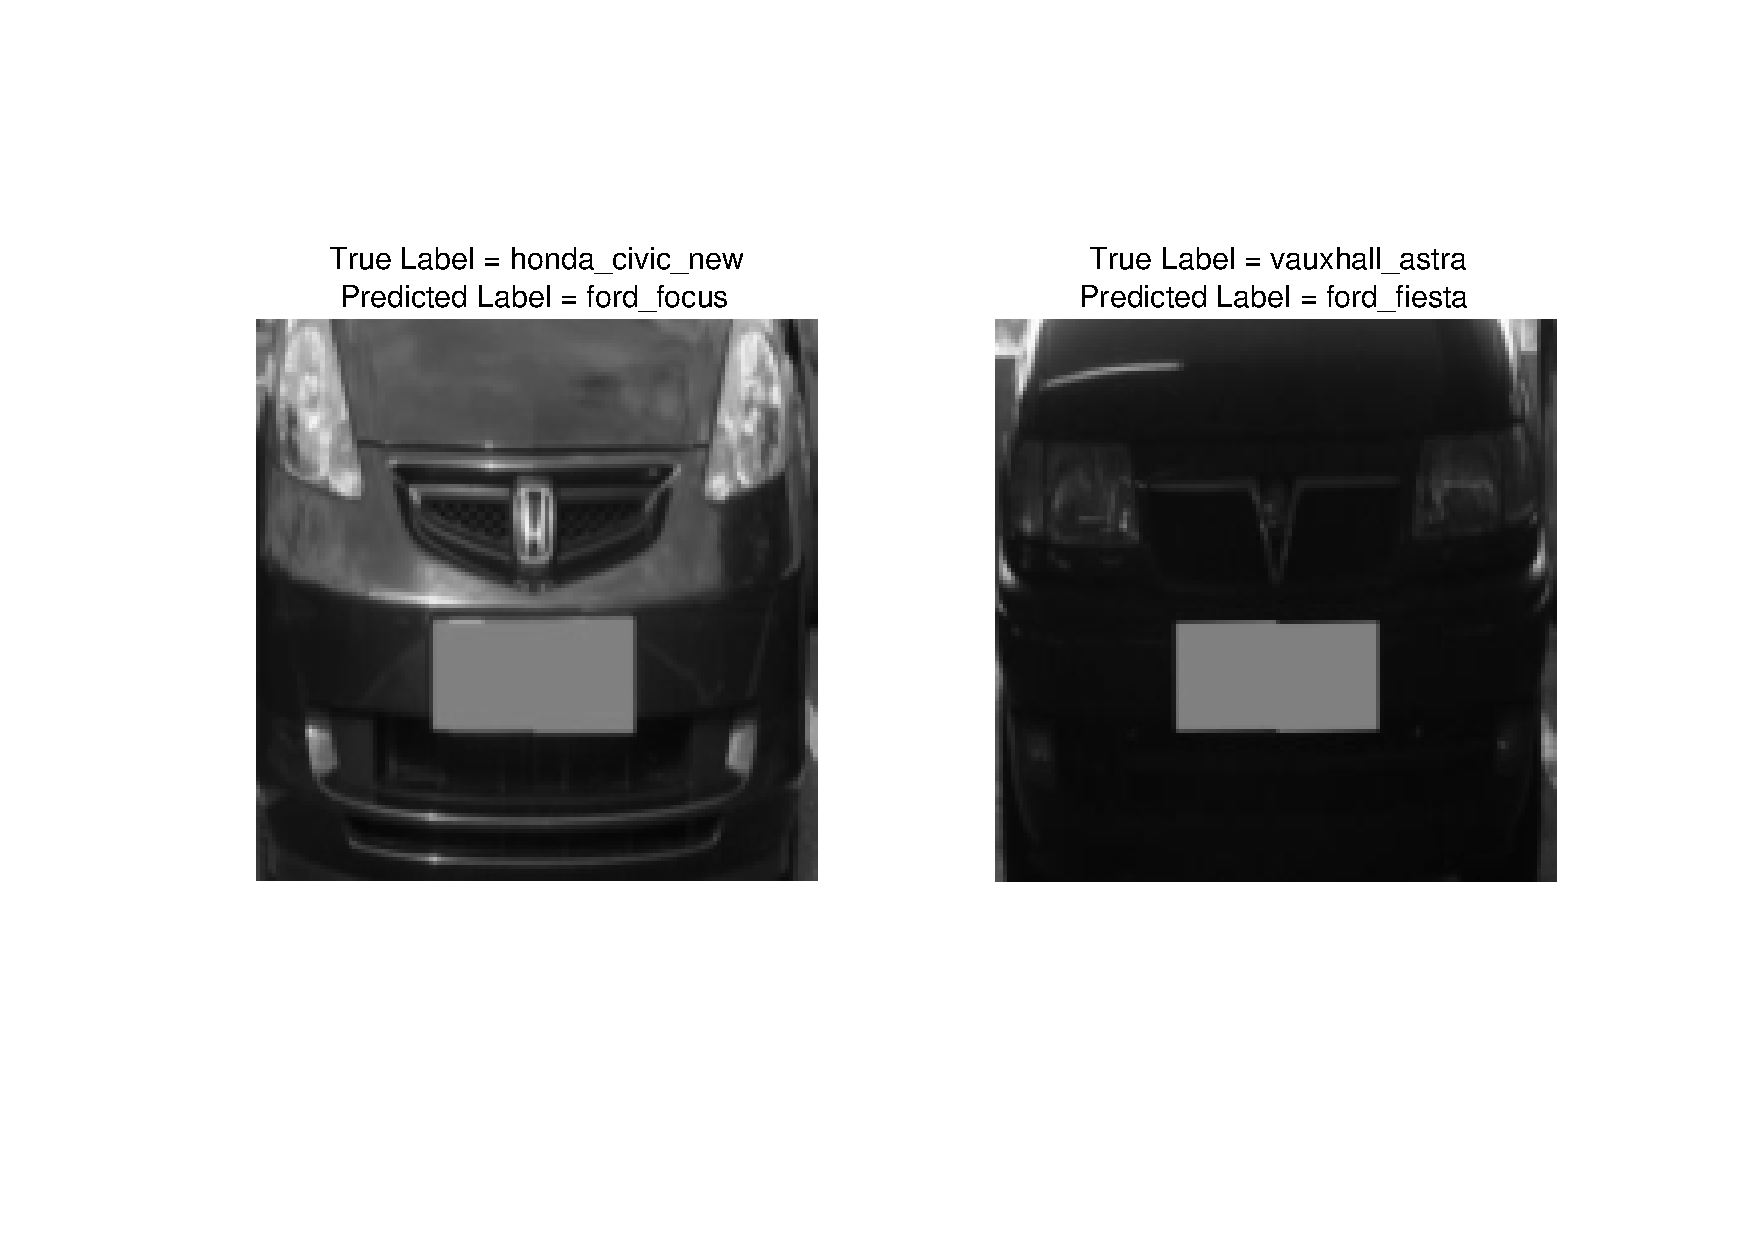
\includegraphics{mis}
\caption{Misclassifications on Corss-Validated Dataset of Our Poposed VMMR System (SMG + PCA + SVM).}
\label{fig:mis}
\end{figure}


